\section{Results}
\label{sec:results}

\subsection{Joint misses exceed the independence prediction}
\begin{figure*}[t]
\centering
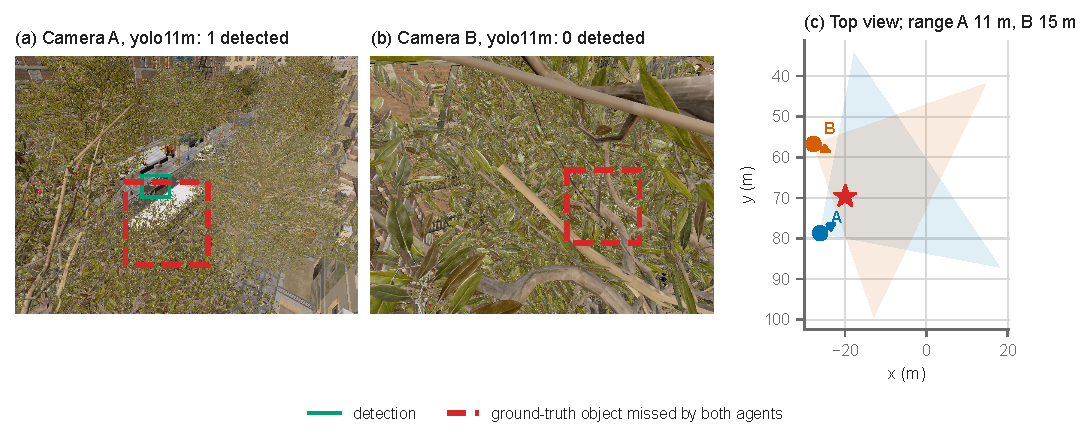
\includegraphics[width=\textwidth]{figures/double_fault_demo}
\caption{One double fault from the 900-scene corpus (scene-0515, medium
viewpoint, static occluder, CloudySunset). A bus, dashed red, is visible to both
agents in the ground truth and is detected by neither YOLO11m run. Green boxes
are detections. Camera~B has none, and the single detection in Camera~A does not
match the bus (IoU below 0.3). Foliage hides the bus from Camera~B and
partly covers it in Camera~A. (c)~Top view in the simulator frame: camera positions,
headings and 90$^\circ$ fields of view; the star is the bus's ground position
from the box bottoms. This is the largest object missed by both agents in the
homogeneous YOLO11m pairing, chosen as an illustration and not as a typical
case.}
\label{fig:double-fault}
\end{figure*}

Table~\ref{tab:calib} reports the practice-scene ratios and the exam-scene
joint miss rates for the random split. Each pairing misses jointly far more
often than the naive product predicts. The calibrated prediction lands within
0.007 of the observed rate for all three pairings.

\begin{table}[t]
\centering
\caption{Random split, 450 practice / 450 exam scenes, 4{,}068 co-visible
exam objects. Ratio is fitted on practice scenes. Joint-miss columns are exam
rates.}
\label{tab:calib}
\footnotesize
\setlength{\tabcolsep}{3pt}
\begin{tabular}{@{}lcccc@{}}
\toprule
Pairing & Ratio $\ratio$ [95\% CI] & Obs. & Calib. & Naive \\
\midrule
YOLO / YOLO       & 1.80 [1.73, 1.87] & 0.241 & 0.238 & 0.133 \\
RT-DETR / RT-DETR & 2.52 [2.38, 2.67] & 0.106 & 0.110 & 0.044 \\
YOLO / RT-DETR    & 1.99 [1.90, 2.08] & 0.141 & 0.148 & 0.074 \\
\bottomrule
\end{tabular}
\end{table}

The RT-DETR-L ratio is the largest, but RT-DETR-L also misses less often
(joint miss 0.106 against 0.241), so its smaller denominator inflates the
ratio. The pairing with the most joint misses in absolute terms is the YOLO11m
pair. Mixing detectors lowers the joint miss rate below the YOLO11m pair
(0.141 against 0.241) without bringing the ratio near 1.
Figure~\ref{fig:double-fault} shows one shared miss.

\subsection{The calibration holds across held-out illumination}
\begin{figure*}[t]
\centering
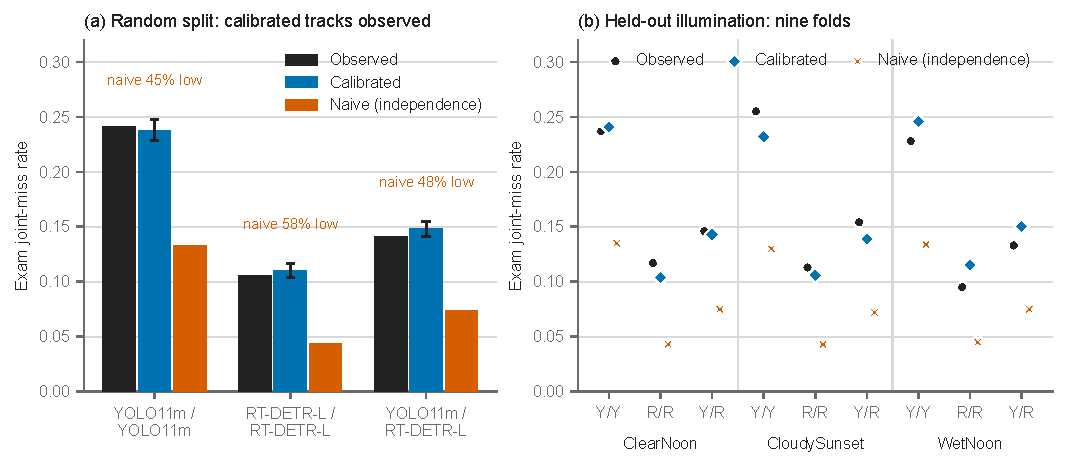
\includegraphics[width=\textwidth]{figures/calibration_stability}
\caption{Exam joint-miss rate: observed, calibrated prediction and naive
independence prediction. (a)~Random split; error bars carry the 95\% interval
of the fitted ratio onto the calibrated prediction. The naive prediction is
45--58\% below the observed rate. (b)~The nine held-out illumination folds
(Y = YOLO11m, R = RT-DETR-L); the naive prediction is 41--63\% below the
observed rate. Values are those of Tables~\ref{tab:calib} and~\ref{tab:shift}.}
\label{fig:calibration}
\end{figure*}

Table~\ref{tab:shift} holds out one illumination at a time (600 practice
scenes, 300 exam scenes). The calibrated prediction stays within 0.025 of the
observed joint miss rate in every case, and is closer than the naive
prediction in all nine. The largest gaps are WetNoon (RT-DETR-L, 0.095
observed against 0.115) and CloudySunset (YOLO11m, 0.255 against 0.232).
An earlier 54-scene dry run failed this test: with ClearNoon held out, YOLO11m
was predicted at 0.273 against 0.103 observed. At 900 scenes the practice
ratios are stable across folds (1.78--1.83 for YOLO11m).
Figure~\ref{fig:calibration} plots both tables.

\begin{table}[t]
\centering
\caption{Shift test: exam joint-miss rate with one illumination held out.
Obs.\ = observed, Cal.\ = calibrated prediction, Naive = independence.}
\label{tab:shift}
\small
\setlength{\tabcolsep}{3pt}
\begin{tabular}{@{}llccc@{}}
\toprule
Held out & Pairing & Obs. & Cal. & Naive \\
\midrule
ClearNoon    & YOLO / YOLO        & 0.237 & 0.241 & 0.135 \\
             & RT-DETR / RT-DETR  & 0.117 & 0.104 & 0.043 \\
             & YOLO / RT-DETR     & 0.146 & 0.143 & 0.075 \\
CloudySunset & YOLO / YOLO        & 0.255 & 0.232 & 0.130 \\
             & RT-DETR / RT-DETR  & 0.113 & 0.106 & 0.043 \\
             & YOLO / RT-DETR     & 0.154 & 0.139 & 0.072 \\
WetNoon      & YOLO / YOLO        & 0.228 & 0.246 & 0.134 \\
             & RT-DETR / RT-DETR  & 0.095 & 0.115 & 0.045 \\
             & YOLO / RT-DETR     & 0.133 & 0.150 & 0.075 \\
\bottomrule
\end{tabular}
\end{table}

\subsection{Decision cost of assuming independence}
\begin{figure*}[t]
\centering
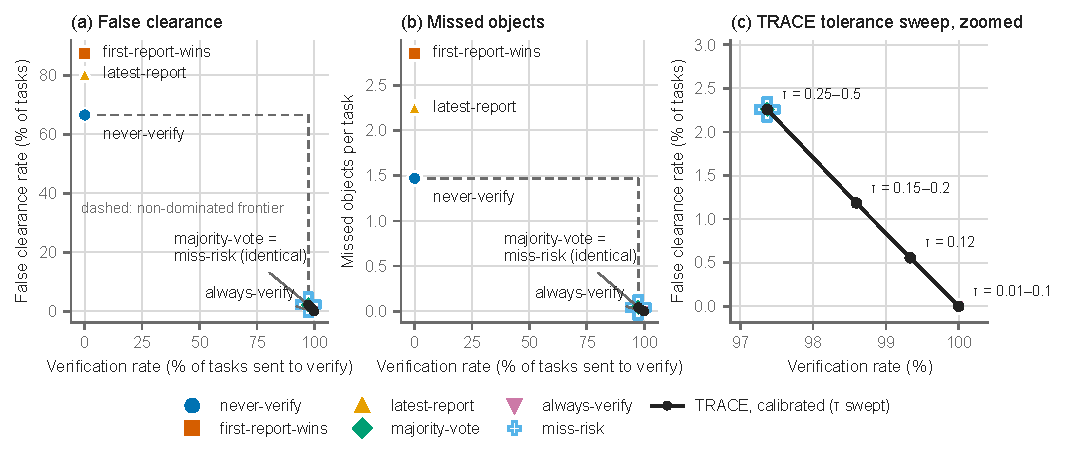
\includegraphics[width=\textwidth]{figures/tradeoffs_pareto}
\caption{Verification rate against risk for six rules and the TRACE tolerance
sweep over the same 2{,}700 tasks. (a)~False clearance rate. (b)~Missed objects
per task. (c)~The sweep, enlarged: miss-risk with the calibrated estimator at 13
tolerances $\tau$ from 0.01 to 0.50. The estimator is fitted on 450 practice
scenes, so half of the tasks are in-sample. Never-verify
closes on the merged tracks of both agents; first-report-wins and latest-report
close on one agent's report; always-verify verifies every task. Majority-vote
and miss-risk v0 give the same counts (61 false clearances, 122 missed objects):
with two agents and the independence estimator, both verify exactly when a
track has a single source. The dashed line joins the rules that no other rule
beats on both axes.}
\label{fig:tradeoffs}
\end{figure*}

Table~\ref{tab:policy} gives the decision outcomes over all 2{,}700 tasks
(5{,}400 decision rows, two per task).

\begin{table}[t]
\centering
\caption{Decision outcomes over 2{,}700 tasks. False clearance: task closed
with at least one co-visible object missed. Both rules used the independence
estimator.}
\label{tab:policy}
\small
\setlength{\tabcolsep}{3pt}
\begin{tabular}{@{}lcccc@{}}
\toprule
Rule & False clear. & Rate & Missed obj. & Verified \\
\midrule
Latest-report & 2{,}172 & 80.4\% & 6{,}084 & 0 \\
Miss-risk v0  & 61      & 2.3\%  & 122     & 2{,}629 \\
\bottomrule
\end{tabular}
\end{table}

Trusting the latest report cleared a task with a missed hazard in four of
five cases. The miss-risk rule cut false clearances from 2{,}172 to 61 tasks
and missed objects from 6{,}084 to 122. It did this by sending 2{,}629 of
2{,}700 tasks (97.4\%) to verification. Of the 71 tasks it closed, 61 still
had a missed object.

Figure~\ref{fig:tradeoffs} places four further rules on the same axes.
It also shows the tolerance sweep. We fitted the calibrated estimator on 450
practice scenes (seed 0) and ran the miss-risk rule at 13 tolerances $\tau$
from 0.01 to 0.50 over all 2{,}700 tasks.

The tolerance has a narrow effect. The single-source test sends 97.4\% of
tasks to verification whatever $\tau$ is. Only the other 71 tasks reach the
risk test. For those tasks the joint miss risk is 0.238 (YOLO/YOLO), 0.110
(RT-DETR/RT-DETR) and 0.148 (YOLO/RT-DETR), so $\tau$ changes a decision only
when it crosses one of these three values. The sweep therefore gives four
points and not a smooth curve (panel~c). At $\tau\le 0.10$ every task is
verified. At $\tau=0.12$ the verification rate is 99.3\% and false clearance
0.6\%. For $\tau$ from 0.15 to 0.20 the values are 98.6\% and 1.2\%. From
$\tau=0.25$ they are 97.4\% and 2.3\%, the same as majority-vote. An operator
can choose among these four settings. Together they span 2.6 points of
verification rate. The 450 exam scenes alone give the same four steps (false
clearance 0.5\%, 1.1\%, and 2.3\%).

The sweep does not show that dependence awareness helps. At $\tau=0.12$ the
rule closes 18 tasks, and 15 of them hold a missed object. Closing 18 tasks
chosen at random from the 71 would leave 15.5 on average. At $\tau=0.15$ the
rule closes 38 tasks, 32 unsafe, against 32.6 for random choice. The
estimator ranks the three detector pairings. It does not rank tasks inside a
pairing. We claim no advantage over naive closing at equal verification
cost.

\subsection{Preliminary 54-scene study}
An earlier study with one YOLO11m across 54 scenes and 448 co-visible objects
gave $\ratio=1.671$ (95\% CI $[1.500,1.870]$). A permutation control that
shuffled one agent's error flags, keeping both marginals fixed, returned
0.999 when the two agents saw different scenes and 1.197 for the same scene
but different objects. About 71\% of the excess attached to the two agents
viewing the same individual object and about 29\% to scene-wide conditions.
These figures come from a smaller corpus and a single detector.
